\chapter{DepthPose}
%% WHAT IS IMPLEMETED
%% WHY DOES IT REPRESENT A PROGRESS IN RESEARCH

%% Objective of the system
The DepthPose here introduced is a complete system for extracting human 3D poses from a single depth image in real-time\footnote{Real-time is defined as being capable of processing at least 30 depth frames per second on the specified minimum hardware requirements.}. It is specifically tailored for use in robotic applications where computational resources are limited. Because the \gls{mecs} is envisioned to be a mobile unit, DepthPose has to be robust to be able to see the person from different viewing angles despite possible occlusions between the person and the depth-sensor. The architecture is inspired by and builds on the architecture in OpenPose~\cite{cao2019openpose}. The general pipeline of DepthPose follows the OpenPose pipeline in figure~\ref{fig:openpose_pipeline} closely, with the addition of a novel Articulation Network that refines the poses after the bipartite matching.

%% Why 3D?
One of the goals for the \gls{mecs} project is to look for patterns that could lead to worsening or more dangerous living conditions. To that end, \gls{har} is implemented with the purpose of tracking a user from day to day. Representing the pose in 3D will simplify application areas such as \gls{har}, because a 3D representation of a skeleton can be defined by a coordinate system constrained to any two connected limbs from the observed skeletons. This means that two different skeleton observations can be represented by a common reference point. Had the skeletons been represented in 2D, the same skeleton seen from two different angles could look vastly different, even if referenced from the same limb. Comparing the two 2D poses will therefore be a more difficult problem than comparing the same poses referenced from a common 3D coordinate system.

%% TODO> about not needing a full 3D body mesh, and privacy concerns


\section{Architecture}

The system pipeline is outlined in figure~\ref{fig:arch_main}. As in \cite{cao2019openpose}, two stages are used to extract the pose from an image. In each stage, a \gls{rnn} architecture iteratively refines the output from the network at that stage. This iterative architecture was inspired by Convolutional Pose Machines~\cite{wei2016cpm}.

At timestep $t = 0$ in the first stage, a set of depth features are created by the first \gls{cnn}, $df$. These are stacked with the \emph{limb-maps} produced by the next \gls{cnn}, $lp$. At $t = 0$ these limb-maps will be initialized to a known value, \textbf{0}, so only the learned bias weights influence $lp$ at this timestep. $lp$ will then refine these limb-maps at subsequent timesteps $0 < t \leq T_{P}$.

At timestep $t = T_{P} + 1$ the refined ``first guess'' limb-maps from $lp$ are again stacked with the depth features from $df$, and used as inputs to $jp$ which produces a set of likely \emph{joint-maps}. These joint-maps are then passed to the Assembly function, which performs the bipartite matching algorithm and constructs a set of skeletons. An instance of the Articulation Network is created for each of the detected skeletons. The Articulation Networks refine the poses for each of the detected skeletons. The refined skeleton poses are then projected onto a set of limb-maps which is used instead of the ``first guess'' limb-maps from $lp$, in successive timesteps $T_{P} + 1 < t \leq T_{P} + T_{C}$.

%% As in \cite{cao209openpose}, two networks are used to create the \gls{paf}s and the confidence maps for the joints. However, instead of training on 3-channel RGB images, we will use a single channel depth image to discover the body landmarks/joints.
%% However, since depth images are single channel, and thus have less information than the RGB images, we propose using a shallower network. This also means we have to do the first step of feature extraction which was already done in a
%% However, since the depth images are less detailed than normal RGB images, some landmarks might be harder to detect: eyes, nose, or placing the joint on an outstretched limb.

%% TODO> about shallowness of network

%% The architecture of this project is \emph{recurrent} in that it repeats itself for a number of iterations. As with the architecture in \cite{cao2017realtime}, we have to have a first step which produces the first outputs we can use in later steps. However, this step is not illustrated in Fig.\ref{fig:arch_main}, since the first step will be identical to the next steps, except it will not have the additional inputs produced by the outputs of the previous step.

\begin{figure}[h]
  \centering
  \includegraphics[width=\textwidth]{img/architecture_main}
  \caption[Main architecture]{Main architecture, as in \cite{cao2017realtime} two recurrent stages, $\phi^{t}$ and $\rho^{t}$ are used to iteratively refine the limb and joint locations.}
  \label{fig:arch_main}
\end{figure}

\subsection{Depth feature extraction}\label{subsec:depth_feature}

\begin{figure}[h]
  \centering
  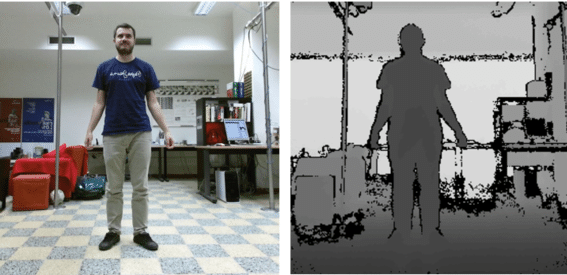
\includegraphics[width=.9\textwidth]{img/rgbd_example}
  \caption[RGB-D Example]{Example of an RGB image on the left vs. a comparative depth image of the same scene on the right. Excerpt sourced from \cite{phdthesisMaxime}.}
  \label{fig:rgbdex}
\end{figure}

The main task for the \gls{cnn} $df$ is to find useful depth features for the subsequent networks. As illustrated in Figure~\ref{fig:rgbdex}, the information in depth images is not as dense as in RGB images. With the goal of object recognition, networks that are trained on RGB images could rely on features such as colors and textures. For example, the blue shirt vs. the khaki pants or the checkerboard pattern of the floor. However, none of those features are present in the depth image. In both images, edges could be extracted to indicate the outline of objects. Indeed, the edges detected in the depth image could be more useful for this purpose than in the RGB image because they would represent the actual 3D boundary between two objects. A quick example could be two boxes of the same color placed partly behind each other. In an RGB image, they could appear to be part of the same object, whereas a sharp edge would separate them in a depth image. Still, much of the information in depth images have to rely on gradients and other features at a larger scale. It can be speculated that representations for planes geometric or organic shapes will be learned.

Figure~\ref{fig:point_cloud} shows that depth images can also be represented as points in a volume. However, to use such a representation of the data as input to a 3D \gls{cnn}, a limit would have to be placed on the observed depth to define a fixed input size. This would lead to a sparse representation of the data, where many convolutions would contain empty space. Since no information can be gathered in the occluded parts of the scene anyway, a single channel depth image is a more succinct representation of the input.

As discussed in Section~\ref{sec:background_cnn}, the feature extraction parts of a network can be trained on large, unrelated datasets. However, no models that were pre-trained on depth images were found, so applying transfer learning for this part of the network was not an option. This part of the model is therefore not necessarily optimal, and having only seen the inside of a dome, it might not have found features that would perform better in a real-world environment.

\begin{figure}[h]
  \centering
  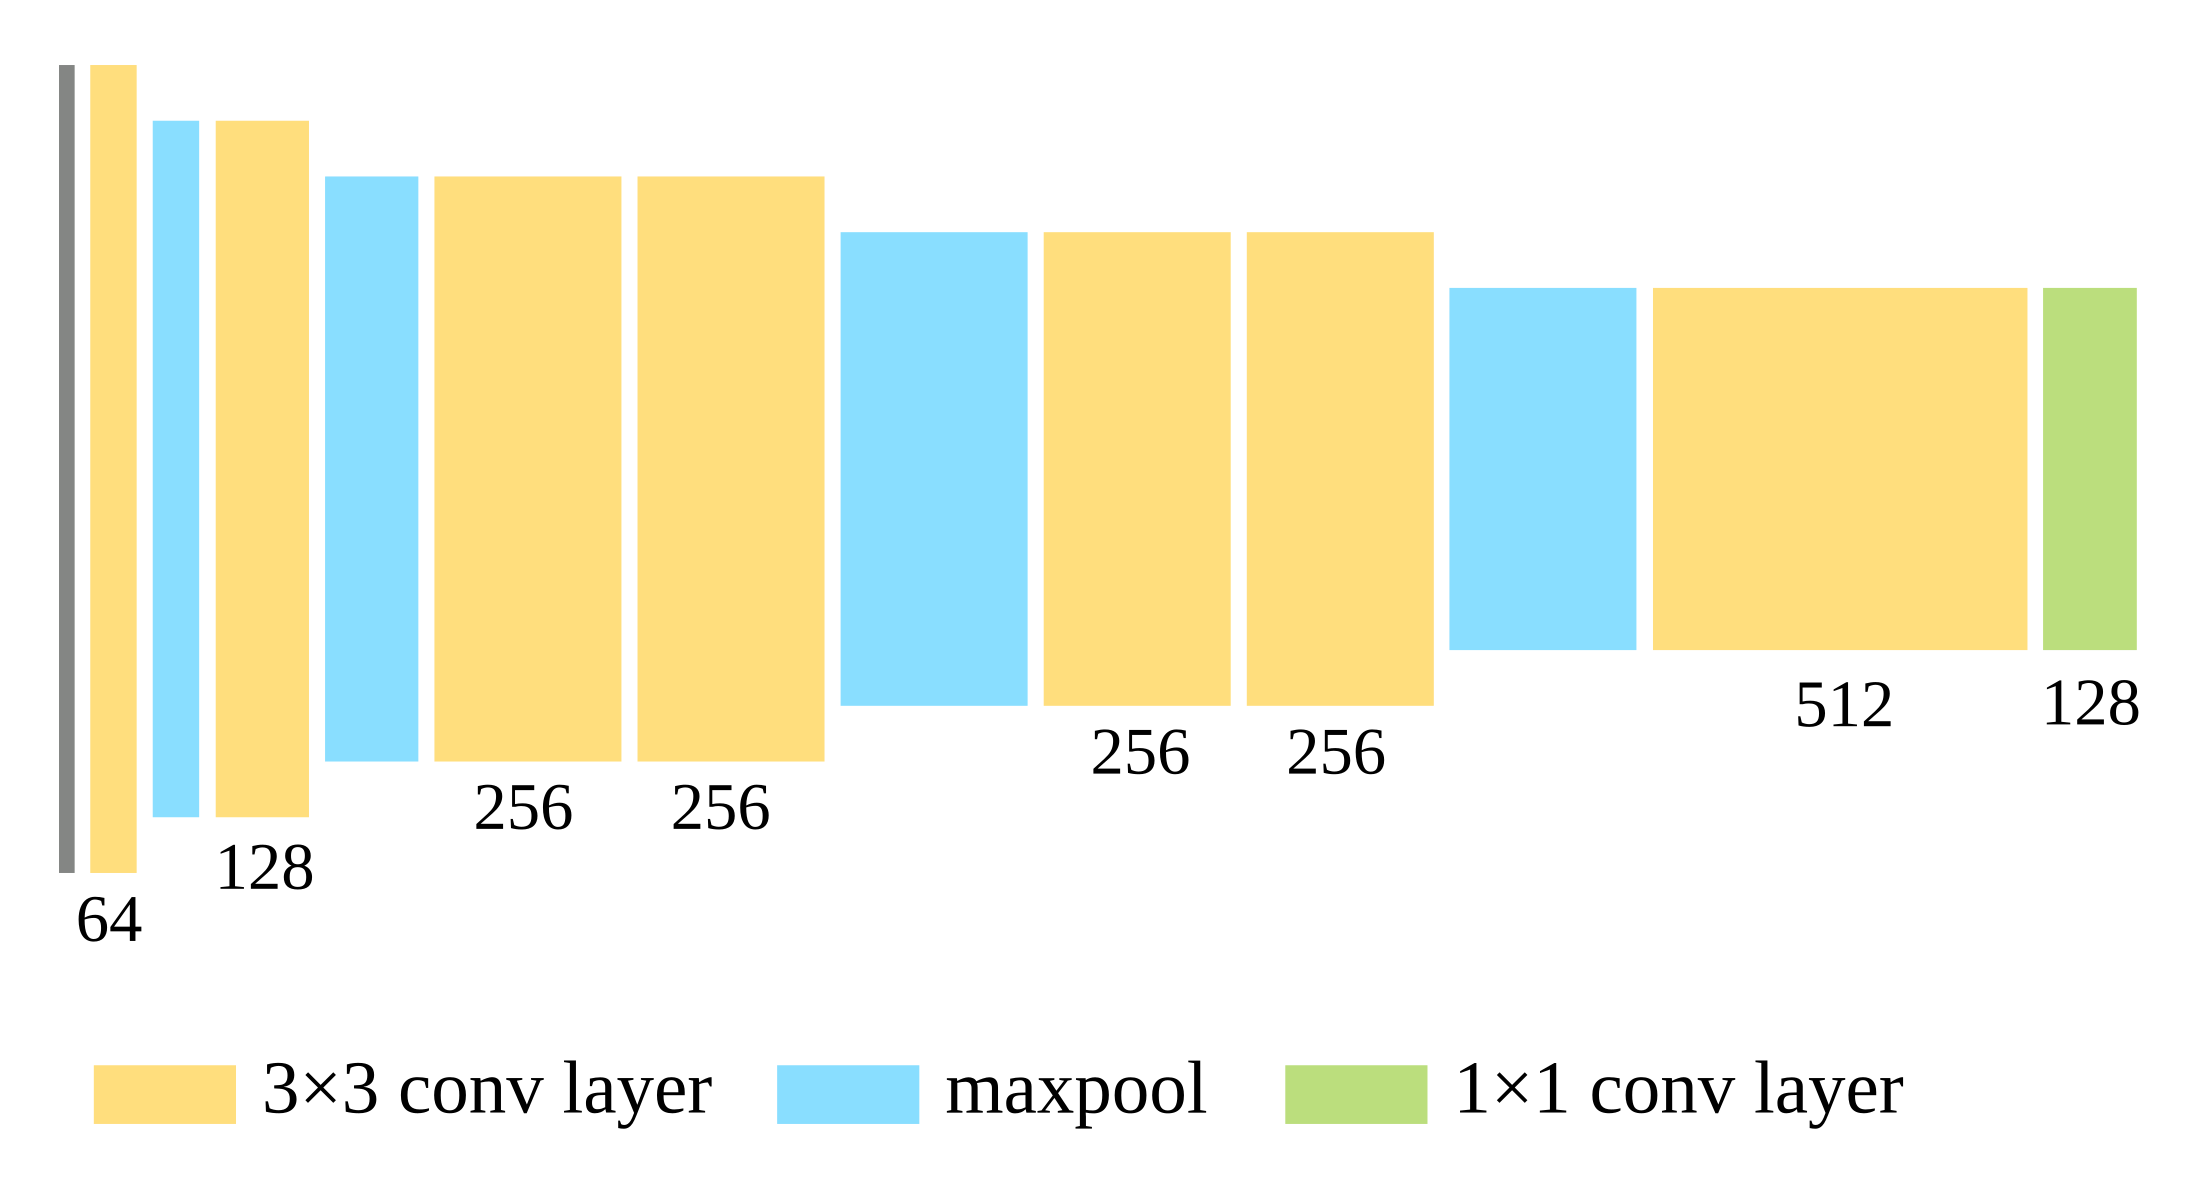
\includegraphics[width=.7\textwidth]{img/convvgg}
  \caption[Depth Feature Extraction]{Depth feature extractor network. The maxpool layers has size $2 \times 2$ and stride 2. Each convolutional layer uses the \gls{relu} activation function.}
  \label{fig:depth_feature_network}
\end{figure}

The OpenPose architecture reuses the first 10 layers of VGG-19 (E configuration)~\cite{simonyan2015deep}. Therefore, this part of the network takes inspiration from it as well. VGG-19 is constructed using several $3 \times 3$ convolutional layers with \gls{relu}~\cite{nairHintonRelu} activations, and maxpool operations at certain depths. By only using enough $3 \times 3$ convolutional layers, the number of learnable parameters are kept down, while preserving the receptive field of a larger kernel (not stacked)\footnote{For an input and output consisting of two channels the learnable parameters can calculated: One $7 \times 7$ kernel $\rightarrow 7^{2}C^{2} = 49C^{2}$ parameters. Three stacked $3 \times 3$ kernels $\rightarrow 3(3^{2}C^{2}) = 27C^{2}$ parameters.}. This is ideal for keeping the network as small, and thus as fast as possible. However, since the information at a small scale can be sparse in depth images, dilation is used to obtain a larger receptive field for each convolutional layer. This is different from pooling layers, because they emit which \emph{feature} in a certain layer has the strongest, weakest or calculate what the average response to the input was. On the other hand, a dilated convolutional layer \emph{creates} features for a larger receptive field, and does not downscale the spacial dimensions of the feature tensor, if same-padding is utilized. The first convolutional layer in Figure~\ref{fig:depth_feature_network} uses dilation of 4 to compensate for the lack of small-scale features in the depth image.

%% \begin{table}
%%   \centering
%%   \begin{tabular}[h]{|c|c|}
%%     \hline
%%     Depth Features $df$ & Limb/Joint Maps $lp$/$jp$ \\
%%     \hline
%%     \hline
%%     Depth image & Features+$lm$ \\ \hline
%%     conv3-64 & conv3 \\ \hline
%%     maxpool & conv3 \\ \hline
%%     conv3-128 & conv3 \\ \hline
%%     maxpool & conv3 \\ \hline
%%     conv3-256 & conv3 \\ \hline
%%     conv3-256 & conv3 \\ \hline
%%     maxpool & conv3 \\ \hline
%%     conv3-256 & conv3 \\ \hline
%%     conv3-256 & conv3 \\ \hline
%%     maxpool & conv3 \\ \hline
%%     conv3-512 & conv3 \\ \hline
%%     conv3-512 & conv3 \\ \hline
%%     conv1-128 & conv3 \\ \hline
%%   \end{tabular}
%%   \caption{\gls{cnn}s presented in this work. \gls{relu}s are omitted for brevity.}
%%   \label{tab:cnns}
%% \end{table}

\begin{figure}[h]
  \centering
  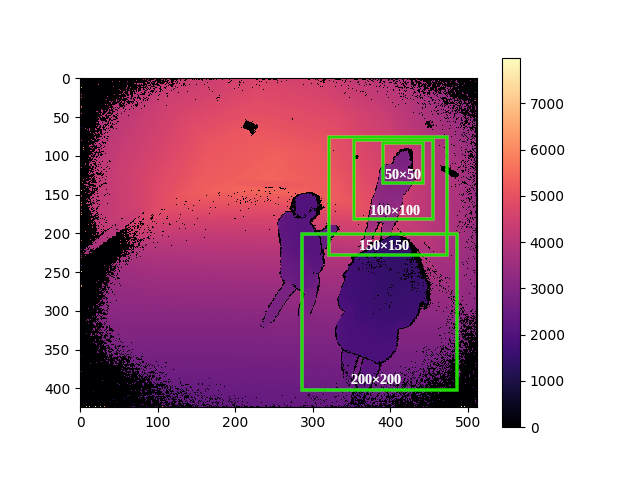
\includegraphics[width=.7\textwidth]{img/depth_image_receptive_fields}
  \caption[Receptive fields in depth images]{Relevant receptive fields in a depth image. Fields are shown as green boxes, with sizes placed near the edge.}
  \label{fig:depth_fields}
\end{figure}

\subsection{Limb- and Joint-Maps}

In \cite{cao2019openpose,wei2016cpm} it is observed that the receptive field of the convolutions are important to establish long-range inferences about body landmarks. This might be because the network learns about the natural symmetries in the human body, and can therefore more easily predict the relationship between different body parts.

In the revisited version of OpenPose, the $7 \times 7$ convolution blocks in the pipeline are replaced by convolution blocks of three $3 \times 3$ filters, where the emissions from each filter is concatenated at the end of the block. This preserves the receptive field of the convolution block, while reducing the number of learnable parameters, as noted in \cite{simonyan2015deep}. In addition, by concatenating the result from each layer at the end of the block, a type of residual network~\cite{he2015deep} is created, mitigating the vanishing gradient problem.

DepthPose uses three such convolution blocks, with a two final $1 \times 1$ convolution layers with dropout between them. This final feature vector is then upsampled through a transposed convolution layer. The output of this is a tensor of $w \times h \times N$ where $N$ is the number of feature maps needed for the network. Since the limb and joint maps look for the same kind of long-reaching features, the architecture is similar.

The limb-map network produce tensors $3M \times w \times h$ where $M$ is the number of limbs in a skeleton. Each limb has 3 components, as they encode the vector pointing in the direction of the limb at that coordinate.

The joint-maps are tensors $2N \times w \times h$ where $N$ is the number of joints in a skeleton. The tensors encode the depth of the limb at that location, as well as the confidence.

%% For each pixel in the current layer of the \gls{cnn}, we collect information from a filter-sized portion of the previous layer. This means that deeper layers look at a larger and larger portion of the input layer. This is useful for detecting connections between large-scale structures. This also means that after a certain depth, there may not be any more useful information.

%% In our experiments, we will try different depths for feature extraction.

%% Some of these features might be desirable as inputs for later layers in object classification.

%% This network is built from the ground up. Therefore we want some layers to, for example, detect edges and one for detecting slanting gradients or connected surfaces. For limbs, we might want to find surfaces that are shaped like tubes or oblong spheroids.

\subsection{Articulation network}\label{subsec:articulation}
The articulation network solves the problem where two people occludes the other. If a joint of the same body part for two people is co-linear to the camera, this joint can not be represented in the joint-map for the occluded person.

The articulation network is stacked on top of the part-detection network and its main role is to refine the limb lengths and angles between each joint. Each of the detected persons are passed through the articulation network, which leads to a bit more complexity and runtime for the network based on the number of people. However, since the network has so comparatively few inputs, and is quite shallow, preformance is not expected to suffer notably.

The coordinates and confidences for each joint (if not detected, confidence is 0) is the input to the network. The network will try to find out what the positions of joints with low confidences, or no detections, should be. It is hypothesized that this network will learn things like symmetry (left and right limbs should have the same length), proportionality (limbs should be proportional to each other), possible articulations, and natural poses.

The architecture is visualized as a simple, almost fully connected neural network. Since each joint has four properties, (x, y, z, c), these are input to a single neuron in the network. The layers after this is however fully connected.

\section{Assembly}

To assemble the poses, candidate points for joints are found by dilating each joint map to find candidate opints. Each of the candidate points are matched up with the corresponding candidate joints following the limb graph. Then, the line integral~\ref{eq:lineint} (line sum, since the sampled pixels are discrete) is taken along the line between the candidate points, however the values for the integral is taken from the corresponding predicted limb map for the joints.
\begin{equation}
  \label{eq:lineint}
  S = \sum_{i=0}^{K}\cos(\theta)
\end{equation}
$\theta$ is the angle between the the vector defined by the candidate points and the angle of the vector at the points of the limb-maps along the line $i, K$. The highest scoring integral is the one chosen as the 'correct' connection. After all the limbs have gotten candidate joints, the predicted skeletons are sent to the articulation network.

\begin{figure}[h]

  \begin{floatrow}
    \ffigbox{
      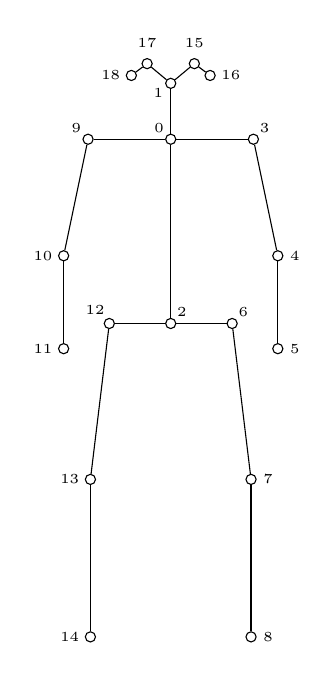
\begin{tikzpicture}[
          every node/.style={draw,circle,minimum size=.06cm, inner sep=1.3pt}
        ]
        \tiny
        %% \draw[help lines, step=5mm, gray!20] (-4,-4) grid (3,4);
        %% Standard coordinates => (orig.coords) - (0, .2)
        \node[label={[label distance=-.2mm]140:{0}}] (neck) at (0,2.54) {};
        \node[label={[label distance=-.2mm]200:{1}}] (nose) at (0,3.25) {};
        \node[label={[label distance=-.2mm]50:{2}}] (mhip) at (0, .2) {};

        \node[label={[label distance=-.2mm]50:{3}}] (lshoulder) at (1.05,2.54) {};
        \node[label={[label distance=-.1mm]0:{4}}] (lelbow) at (1.36,1.06) {};
        \node[label={[label distance=-.1mm]0:{5}}] (lwrist) at (1.36,-.12) {};
        \node[label={[label distance=-.2mm]50:{6}}] (lhip) at (.78,.2) {};
        \node[label={[label distance=-.1mm]0:{7}}] (lknee) at (1.02,-1.78) {};
        \node[label={[label distance=-.1mm]0:{8}}] (lankle) at (1.02,-3.78) {};

        \node[label={[label distance=-.2mm]140:{9}}] (rshoulder) at (-1.05,2.54) {};
        \node[label={[label distance=-.1mm]180:{10}}] (relbow) at (-1.36,1.06) {};
        \node[label={[label distance=-.1mm]180:{11}}] (rwrist) at (-1.36,-.12) {};
        \node[label={[label distance=-.2mm]140:{12}}] (rhip) at (-.78,.2) {};
        \node[label={[label distance=-.1mm]180:{13}}] (rknee) at (-1.02,-1.78) {};
        \node[label={[label distance=-.1mm]180:{14}}] (rankle) at (-1.02,-3.78) {};

        \node[label={[label distance=-.1mm]90:{15}}] (leye) at (.3,3.5) {};
        \node[label={[label distance=-.1mm]0:{16}}] (lear) at (.5,3.35) {};
        
        \node[label={[label distance=-.1mm]90:{17}}] (reye) at (-.3,3.5) {};
        \node[label={[label distance=-.1mm]180:{18}}] (rear) at (-.5,3.35) {};

        %% \draw[blue] (0,0) circle [radius=.06cm];

        \draw (nose) -- (neck);
        \draw (neck) -- (mhip);

        \draw (reye) -- (nose); \draw (leye) -- (nose);
        \draw (reye) -- (rear); \draw (leye) -- (lear);
        
        \draw (neck) -- (rshoulder); \draw (neck) -- (lshoulder);
        %% \draw (neck) -- (rhip); \draw (neck) -- (lhip);
        \draw (neck) -- (mhip);

        \draw (rshoulder) -- (relbow); \draw (lshoulder) -- (lelbow);
        \draw (rwrist) -- (relbow); \draw (lwrist) -- (lelbow);

        \draw (mhip) -- (rhip); \draw (mhip) -- (lhip);
        \draw (rhip) -- (rknee); \draw (lhip) -- (lknee);
        \draw (rknee) -- (rankle); \draw (lknee) -- (lankle);
      \end{tikzpicture}
    }
    {
      \caption[Numbering for keypoint markers]{Numbering for detected landmarks/keypoint markers.}
      \label{fig:skeleton_markers}
    }
    %% \end{figure}
    %% \begin{table}
    \capbtabbox{
      \footnotesize
      \begin{tabular}[H]{|r l r|}
        \hline
        \textbf{ID} & \textbf{Description} & \textbf{Std.Coord.} \\ \hline
        0  & Neck & (0.00, 2.34) \\
        1  & Nose & (0.00, 3.05) \\
        2  & Middle hip & (0.00, 0.00) \\
        3  & Left shoulder & (1.05, 2.34) \\
        4  & Left elbow & (1.36, 0.86) \\
        5  & Left wrist & (1.36, -0.32) \\
        6 & Left hip & (0.78, 0.00) \\
        7 & Left knee & (1.02, -1.98) \\
        8 & Left ankle & (1.02, -3.98) \\
        9  & Right shoulder & (-1.05, 2.34) \\
        10 & Right elbow & (-1.36, 0.86) \\
        11 & Right wrist & (-1.36, -0.32) \\
        12 & Right hip & (-0.78, 0.00) \\
        13 & Right knee & (-1.02, -1.98) \\
        14 & Right ankle & (-1.02, -3.98) \\
        15 & Left eye & (0.30, 3.30) \\
        16 & Left ear & (0.50, 3.15) \\
        17 & Right eye & (-0.30, 3.30) \\
        18 & Right ear & (-0.50, 3.15) \\
        \hline
      \end{tabular}
    }{
      \caption[Names/coordinates for detected landmarks]{Numberings, names/descriptions and standard coordinates for recognized landmarks}
      \label{tab:openpose_body_ids}
    }
  \end{floatrow}          
\end{figure}

\section{Training}
%% criterion, why was this chosen
%% Learning rate
%% optimizer

